\documentclass[a4paper,14pt]{extreport}
\usepackage[left=1.5cm,right=1.5cm,
    top=1.5cm,bottom=2cm,bindingoffset=0cm]{geometry}
\usepackage{scrextend}
\usepackage[T1,T2A]{fontenc}
\usepackage[utf8]{inputenc}
\usepackage[russian,ukrainian,english]{babel}
\usepackage{tabularx}
\usepackage{amssymb}
\usepackage{color}
\usepackage{amsmath}
\usepackage{mathrsfs}
\usepackage{listings}
\usepackage{graphicx}
\graphicspath{ {./images/} }
\usepackage{lipsum}
\usepackage{xcolor}
\usepackage{hyperref}
\usepackage{tcolorbox}
\usepackage{tikz}
\usepackage[framemethod=TikZ]{mdframed}
\usepackage{wrapfig,boxedminipage,lipsum}
\mdfdefinestyle{MyFrame}{%
linecolor=blue,outerlinewidth=2pt,roundcorner=20pt,innertopmargin=\baselineskip,innerbottommargin=\baselineskip,innerrightmargin=20pt,innerleftmargin=20pt,backgroundcolor=gray!50!white}
 \usepackage{csvsimple}
 \usepackage{supertabular}
\usepackage{pdflscape}
\usepackage{fancyvrb}
%\usepackage{comment}
\usepackage{array,tabularx}
\usepackage{colortbl}

\usepackage{varwidth}
\tcbuselibrary{skins}
\usepackage{fancybox}


\usepackage{tikz}
\usepackage[framemethod=TikZ]{mdframed}
\usepackage{xcolor}
\usetikzlibrary{calc}
\makeatletter
\newlength{\mylength}
\xdef\CircleFactor{1.1}
\setlength\mylength{\dimexpr\f@size pt}
\newsavebox{\mybox}
\newcommand*\circled[2][draw=blue]{\savebox\mybox{\vbox{\vphantom{WL1/}#1}}\setlength\mylength{\dimexpr\CircleFactor\dimexpr\ht\mybox+\dp\mybox\relax\relax}\tikzset{mystyle/.style={circle,#1,minimum height={\mylength}}}
\tikz[baseline=(char.base)]
\node[mystyle] (char) {#2};}
\makeatother

\definecolor{ggreen}{rgb}{0.4,1,0}
\definecolor{rred}{rgb}{1,0.1,0.1}
\definecolor{amber}{rgb}{1.0, 0.75, 0.0}
\definecolor{babyblue}{rgb}{0.54, 0.81, 0.94}
\definecolor{asparagus}{rgb}{0.53, 0.66, 0.42}
\definecolor{chartreuse}{rgb}{0.5, 1.0, 0.0}
\definecolor{darkorchid}{rgb}{0.6, 0.2, 0.8}

\usepackage{float}
\usepackage{wrapfig}
\usepackage{framed}
%for nice Code{
\lstdefinestyle{customc}{
  belowcaptionskip=1\baselineskip,
  breaklines=true,
  frame=L,
  xleftmargin=\parindent,
  language=C,
  showstringspaces=false,
  basicstyle=\small\ttfamily,
  keywordstyle=\bfseries\color{green!40!black},
  commentstyle=\itshape\color{purple!40!black},
  identifierstyle=\color{blue},
  stringstyle=\color{orange},
}
\lstset{escapechar=@,style=customc}
%}


\begin{document}
\pagecolor{white}

%----------------------------------------1
\newtcbox{\xmybox}[1][red]{on line, arc=7pt,colback=#1!10!white,colframe=#1!50!black, before upper={\rule[3pt] {0pt}{10pt}},boxrule=1pt,boxsep=0pt,left=6pt,right=6pt,top=2pt,bottom=2pt}

\begin{center}\xmybox[babyblue]{Mnatsakanov Anton} \xmybox[amber]{DP-82} 
\vspace{1cm}

\end{center}


\begin{center}\fbox{\fbox{VIII. Piezoelectrics and their main applications}}
  \end{center}

The piezoelectric effect was discovered in 1880 by brothers Pierre and Jacques Curie; quartz (Fig.~\ref{ris1}), tourmaline, topaz and Rochelle salt have such abilities.
In general, piezoelectrics are such dielectrics (dielectric crystals) in which polarization occurs when mechanical action (compression, stretching) is applied to it. The inverse phenomenon of the piezoelectric effect is electrostriction. One of the best known piezoelectrics is monocrystalline quartz, anhydrous silicon dioxide crystallizing in the trigonal-trapezohedral class of hexagonal syngony. Large natural transparent quartz crystals are called rock crystal. In addition to quartz, lithium niobate and lithium tantalate are commonly used as materials for piezoelectric elements. These materials are inherently ferroelectric. To give them piezoelectric properties, they are annealed in a strong electric field, which leads to a monodomain state.\\
Similarly, segmented ceramics can be converted to the piezoelectric state. Polarized ferroelectric ceramics are called piezoceramics. Piezo-ceramics have the advantage over monocrystals that they can be used to produce an active element of any shape and size. Solid solutions based on barium titanate, lead titanate-zirconate, lead methanobate are used as the material for piezoceramics.\\
\begin{figure}[h]
\center{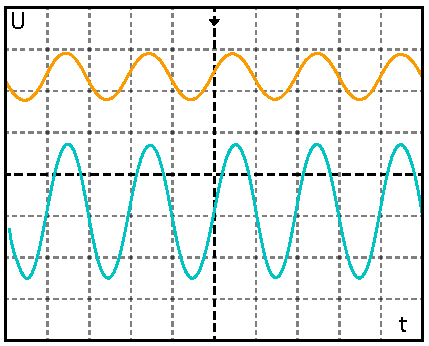
\includegraphics[width=0.5\linewidth]{11.jpg}}
\caption{Quartz monocrystal}
\label{ris1}
\end{figure}


Piezoceramic materials are commonly divided into four functional groups. Group 1 materials are used to manufacture highly sensitive elements operating in the mode of reception or emission of mechanical vibrations. Such materials require a large piezomodulus. Group 2 materials are used for the manufacture of strong signal generators, operating in conditions of strong electric fields or high mechanical stress. Such materials require high specific electrical resistance. Group 3 materials are used to manufacture piezoelectric elements with improved stability of resonant frequencies depending on temperature and time. Group 4 materials are used to manufacture high-temperature piezoelectric elements.\\

Basically 
In generators, piezoelectric materials can generate a voltage that is sufficient to produce a spark between electrodes and can thus be used as electrodes for igniting fuel, for gas stoves and for welding equipment. Alternatively, the electrical energy generated by piezoelectric elements can be stored. Such generators are excellent solid-state batteries for electronic circuits.\\

In sensors, piezoelectric materials convert physical parameters such as acceleration, pressure, and vibration into 
an electrical signal.\\

In actuators, piezoelectric materials convert an electrical signal into a precisely controlled physical displacement, clearly establishing the accuracy of mechanical tools, lenses and mirrors.
In transducers, piezoelectric transducers can both generate an ultrasonic signal from electrical energy and convert incoming mechanical vibrations into electrical vibrations. Piezoelectric transducers are designed to measure distances, flow rates, and liquid levels. Transducers are also used to generate ultrasonic vibrations for cleaning, drilling, welding, grinding ceramics and for medical diagnostics.\\


\begin{figure}[h]
\center{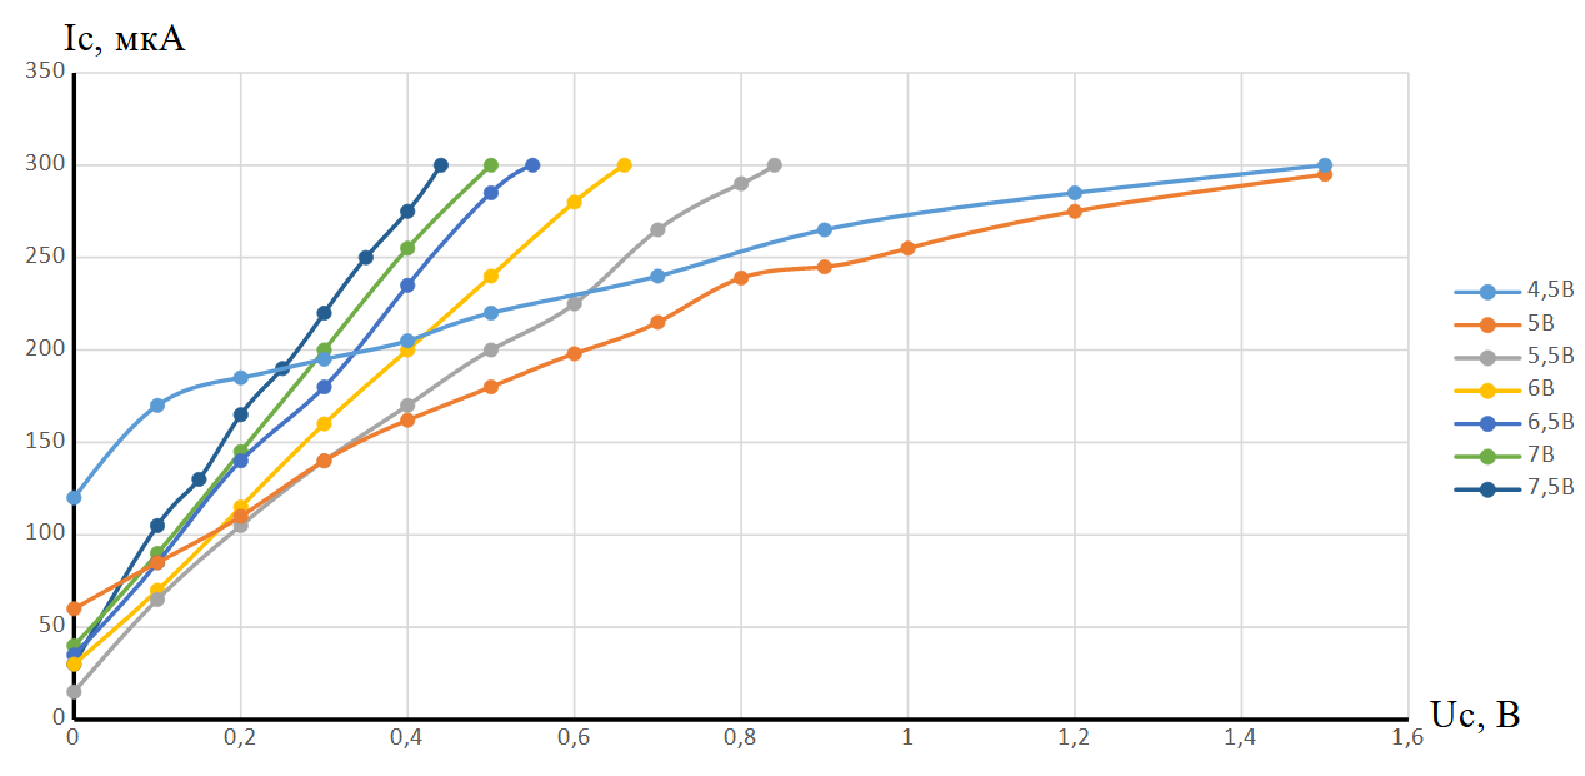
\includegraphics[width=0.55\linewidth]{5.jpg}}
\caption{Frequency dependence of resistance in piezoceramics}
\end{figure}

Here are a few examples:\\

Sonar Equipment — Depth sounders and sonar equipment rely extensively on piezoelectric sensors to transmit and receive ultrasonic “pings” in the 50-200kHz range. Besides having an ideal frequency response for such applications, piezoelectric transducers have a high power density that enables large amounts of acoustic power to be transmitted from a small package. For instance, a transducer that is only 4” (100 mm) in diameter may be capable of handling power output greater than 500 watts.\\
\begin{figure}[h!]
\center{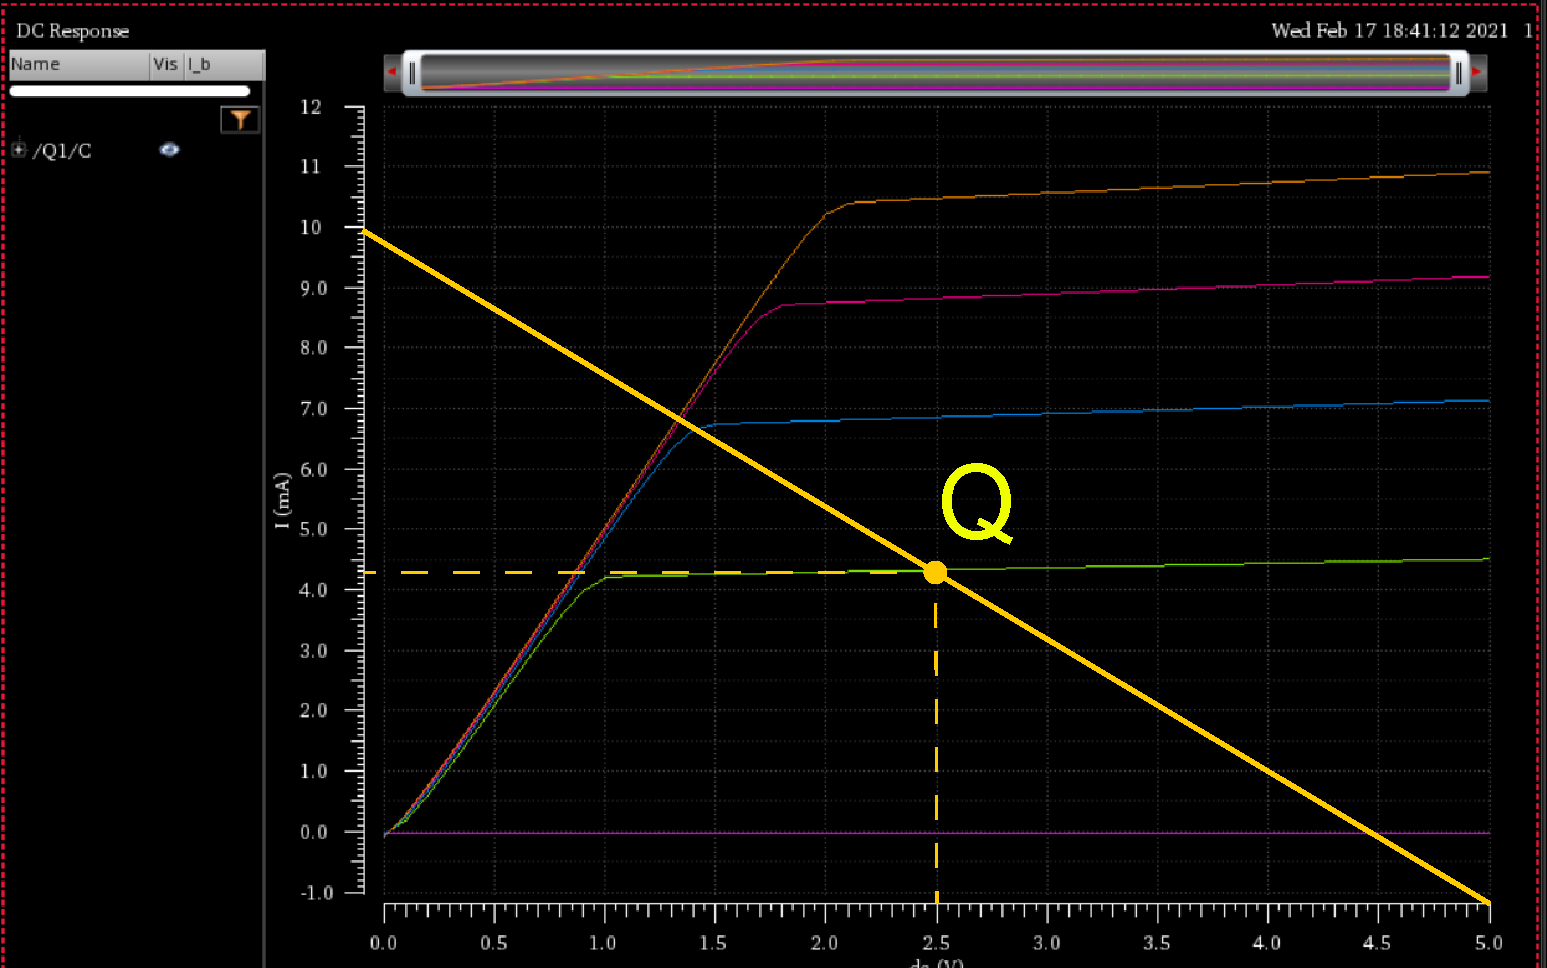
\includegraphics[width=0.4\linewidth]{1.jpg}}
\end{figure}



Pressure Sensors — In nearly any application requiring the measurement of dynamic pressure changes, using piezoelectric pressure sensors yields more reliable results than using conventional electromechanical pressure sensors. This is because piezoelectric devices have a high frequency response and signal conversion without requiring any bellows, diaphragm, or any type of mechanical linkage in conjunction with a strain gage or displacement sensor.\\
\begin{figure}[h!]
\center{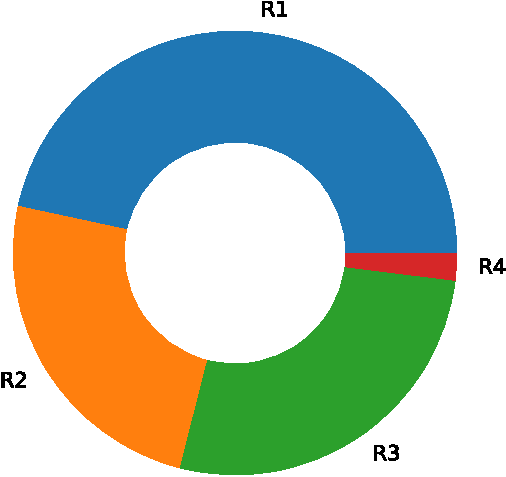
\includegraphics[width=0.3\linewidth]{2.jpg}}
\caption{Pressure sensors in the housing}
\end{figure}

Engine Knock Sensors — Engine manufacturers are constantly facing challenges related to the control of engine parameters. Under the wrong circumstances, gasoline engines are susceptible to an undesirable phenomenon known as detonation. When detonation occurs, the air/fuel charge explodes instead of burning smoothly thereby damaging the engine. Historically, this is why most manufacturers designed engines with conservative operational margins at the expense of efficiency — it was to avoid this notorious problem.\\
\begin{figure}[h!]
\center{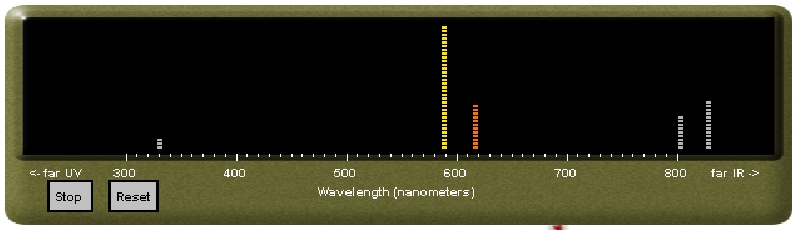
\includegraphics[width=0.5\linewidth]{3.jpg}}
\end{figure}

\newpage
Also piezoelectrics use for Ultrasonic Welding — many plastics, or other material, can be joined together using a process known as ultrasonic welding. This type of process requires ultrasonic waves to be transmitted to a focused area where they can cause pieces of plastic to fuse together. Frequently, piezoelectric actuators are used to accomplish this task.\\
\begin{figure}[h!]
\center{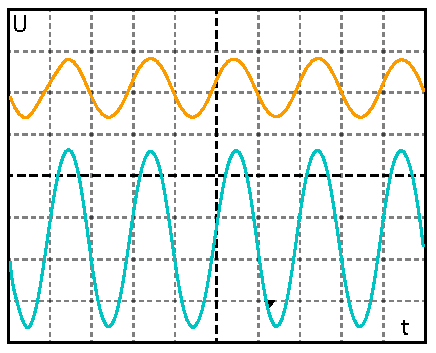
\includegraphics[width=0.6\linewidth]{4.jpg}}
\caption{Application of Ultrasonic Welding}
\end{figure}























\end{document}
